\section{Implementation}
% motivation for creating this theme
\begin{frame}{Designing the Ensemble}{R-FCN ResNet-101}
    \begin{block}{Overview}
    \begin{itemize}
        \item Ensemble of R-FCNs with ResNet-101
        \item Data sampling \& selection
        \begin{itemize}
            \item Object resolution
            \item Image quality
        \end{itemize}
        \item Training member classifiers
        \begin{itemize}
            \item Kept constant
        \end{itemize}
        \item Combining ensemble members
        \begin{itemize}
            \item Average
            \item Weighted Average
        \end{itemize}       
    \end{itemize}
\end{block}
\end{frame}

\begin{frame}{Object Resolution}{Training Members}
        \begin{block}{Subset creation}
        \begin{itemize}
            \item Ground truth bounding box area
            \begin{itemize}
                \item 19,205.5 pixels
            \end{itemize}
            \item RPN proposals bounding box area
            \begin{itemize}
                \item 4,684 pixels
            \end{itemize}
            \item R-FCN trained with proposals inputs
            \begin{itemize}
                \item RPN finds examples
            \end{itemize}
        \end{itemize}
    \end{block}
\end{frame}

\begin{frame}{Object Resolution}{Training Members}
\begin{columns}
    \column{0.3\textwidth}
        \begin{figure}
            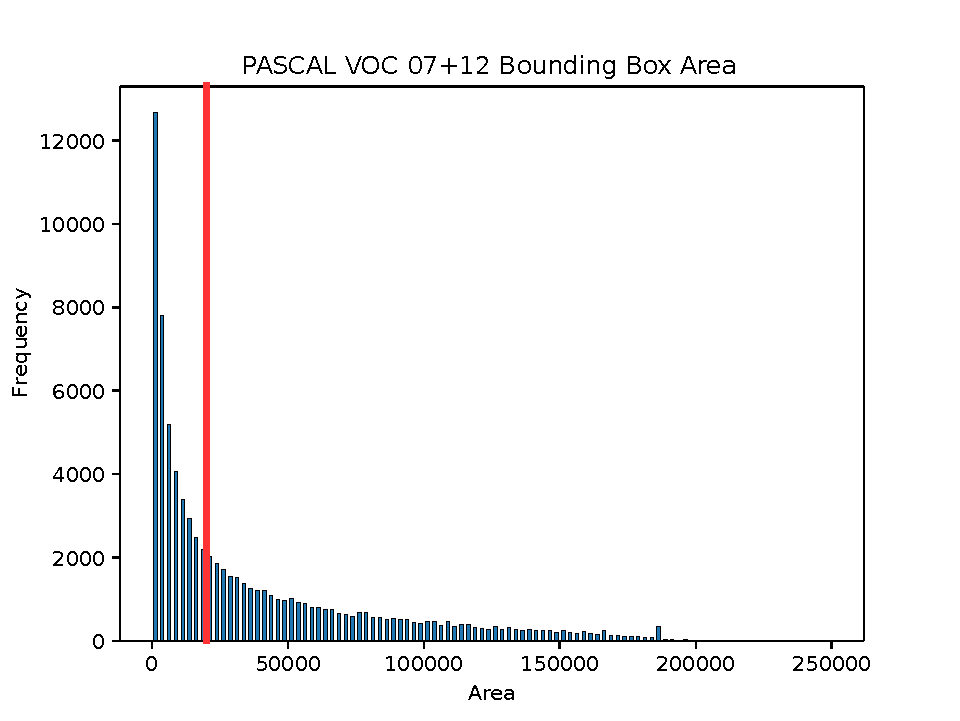
\includegraphics[width=1.4 \textwidth]{figs/trainvalhistred.pdf}
        \end{figure}

 \column{0.7\textwidth}
        \begin{table}[h]
            \centering
            \begin{tabular}{|l|l|l|}
                \hline
                \textbf{Data} & \textbf{RPN$_{small}$} & \textbf{RPN$_{larger}$} \\ \hline
                Ground Truth & 19,992    & 60,116     \\ 
                Background   & 4,969,369 & 4,929,297  \\ \hline
                Total        & 4,989,361 & 4,989,413  \\ \hline
            \end{tabular}
        \end{table}

        \begin{table}[h]
            \centering  
            \begin{tabular}{|l|l|l|}
                \hline
                \textbf{Data} & \textbf{RPN$_{small}$} & \textbf{RPN$_{larger}$} \\ \hline
                Ground Truth & 40,058    & 40,058     \\ 
                Background   & 3,528,370 & 6,370,859  \\ \hline
                Total        & 3,568,428 & 6,410,917  \\ \hline
            \end{tabular}
        \end{table}
        \end{columns}
\end{frame}

\begin{frame}{Object Resolution}{Training Members}
\begin{columns}
    \column{0.3\textwidth}
      \begin{block}{Evaluating experts}
        \begin{itemize}
            \item Initial results promising
        \end{itemize}
    \end{block}
       
    \column{0.7\textwidth}

        
        \begin{table}[h]
        \centering
        \begin{tabular}{|l|l|}
        \hline
        \textbf{Train Data} & \textbf{AP}      \\ \hline
        RPN$_{small}$      & \textbf{55.00\%} \\ \hline
        RPN$_{larger}$      & 20.92\% \\ \hline
        07+12        & 43.80\% \\ \hline
        \end{tabular}
        \end{table}

        \begin{table}[h]
        \centering
        \begin{tabular}{|l|l|}
        \hline
        \textbf{Train Data} & \textbf{AP}      \\ \hline
        RPN$_{small}$      & 21.28\% \\ \hline
        RPN$_{larger}$      & \textbf{81.81\%} \\ \hline
        07+12        & 75.14\% \\ \hline
        \end{tabular}
        \end{table}


        \begin{table}[h]
        \centering
        \begin{tabular}{|l|l|}
        \hline
        \textbf{Train Data} & \textbf{AP}      \\ \hline
        RPN$_{small}$      & 46.74\% \\ \hline
        RPN$_{larger}$      & 62.48\% \\ \hline
        07+12        & \textbf{79.59\%} \\ \hline
        \end{tabular}
        \end{table}


      
    \end{columns}
\end{frame}

\begin{frame}{Image Quality}{Training Members}
\begin{columns}
    \column{0.5\textwidth}
        \begin{block}{Deep IQA}
        \begin{itemize}
            \item VGG-inspired NR-IQA
            \item Trained on LIVE IQA dataset
            \item 5 models trained on distortion types
            \begin{itemize}
                \item Gaussian blur, white noise, JPEG compression, JP2K compression, fast fading bit errors
            \end{itemize}
        \end{itemize}
    \end{block}
    \column{0.5\textwidth}
        \begin{figure}
            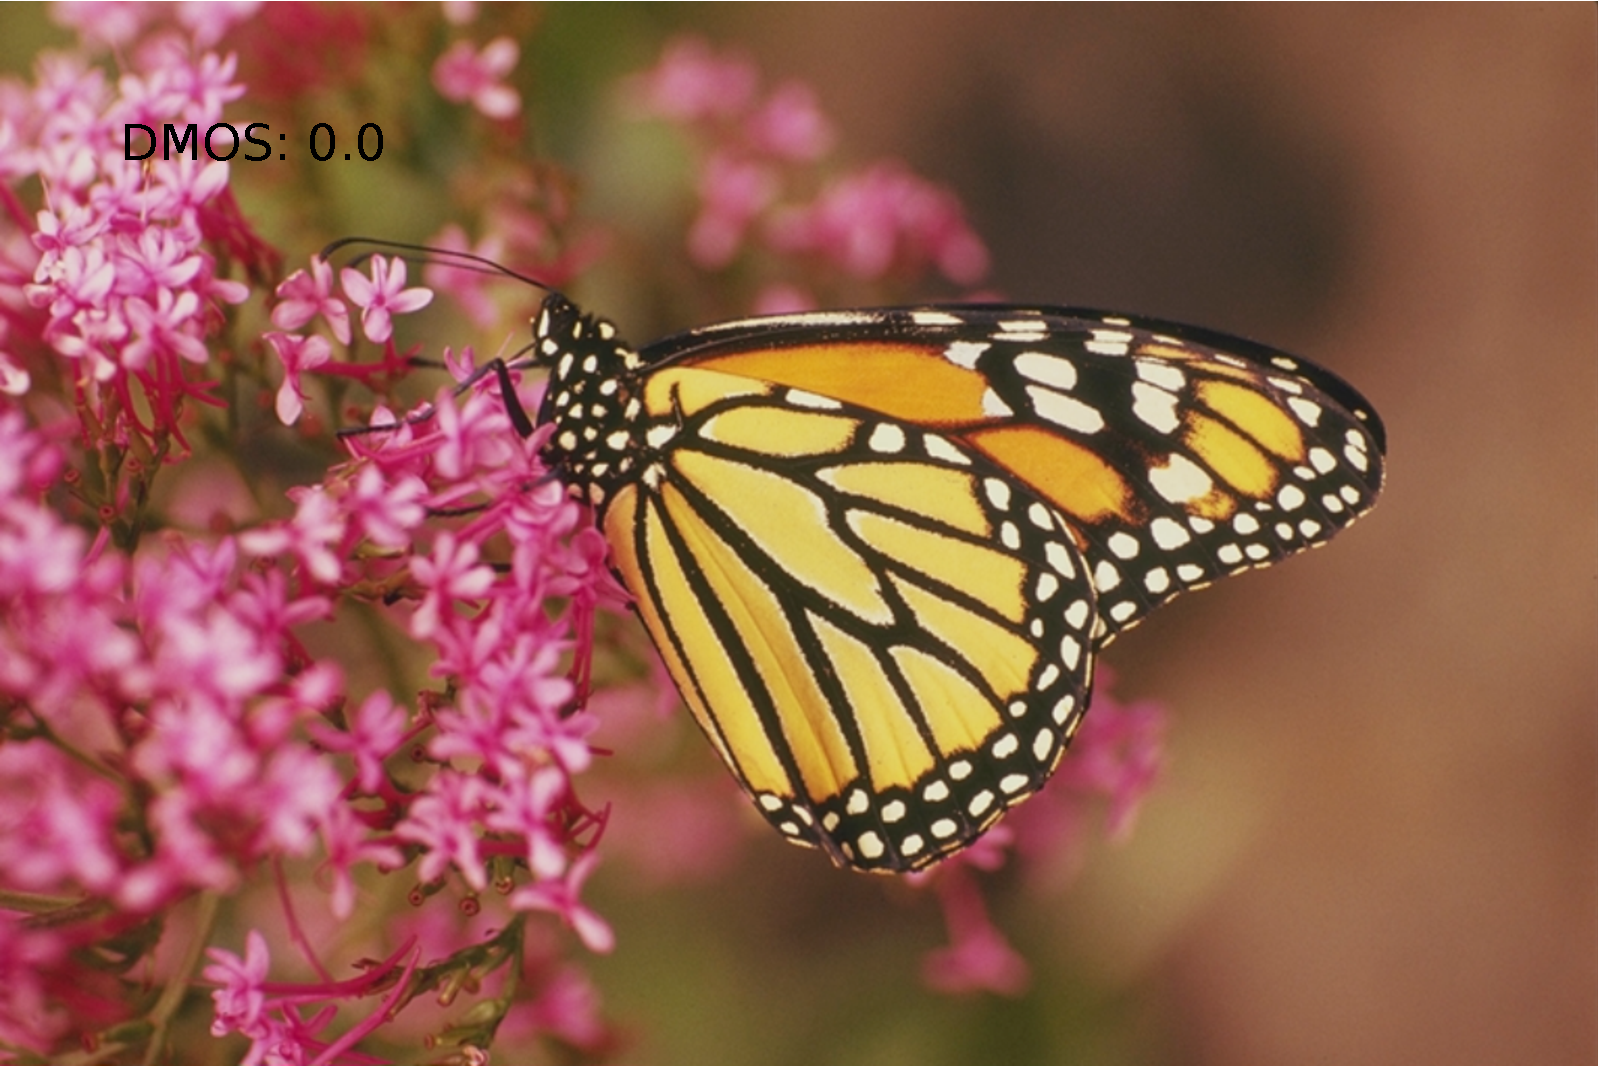
\includegraphics[width=0.5 \textwidth]{figs/img173.pdf}
        \end{figure}
        \begin{figure}
            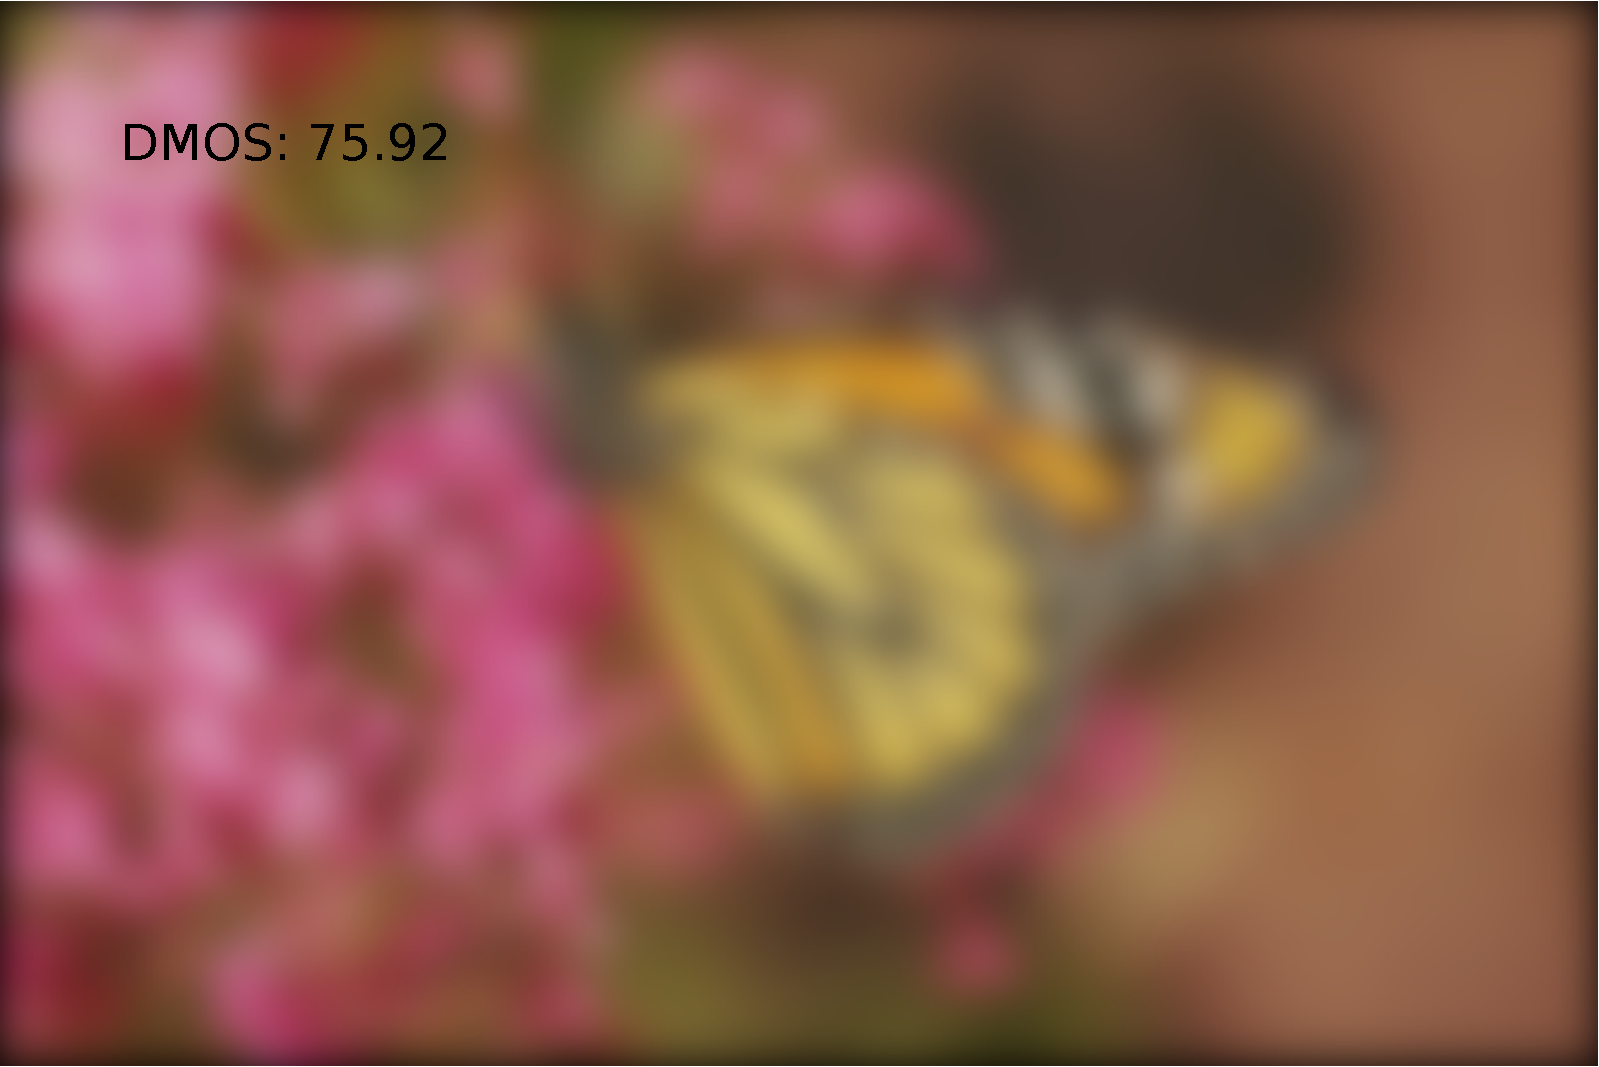
\includegraphics[width=0.5 \textwidth]{figs/img11.pdf}
        \end{figure}
    \end{columns}
\end{frame}

\begin{frame}{Image Quality}{Training Members}
\vspace{-0.5cm}
\begin{columns}

    \column{0.5\textwidth}
    \begin{figure}
        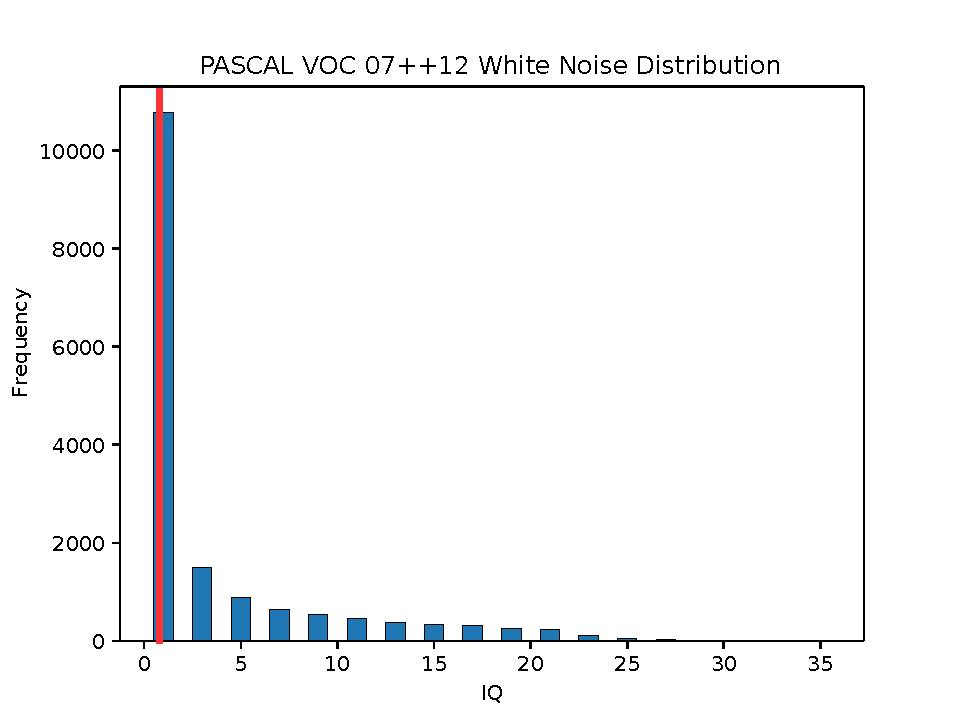
\includegraphics[width=0.5 \textwidth]{figs/WhiteNoisedistred.pdf}
    \end{figure}
    \vspace{-0.5cm}
    \begin{figure}
        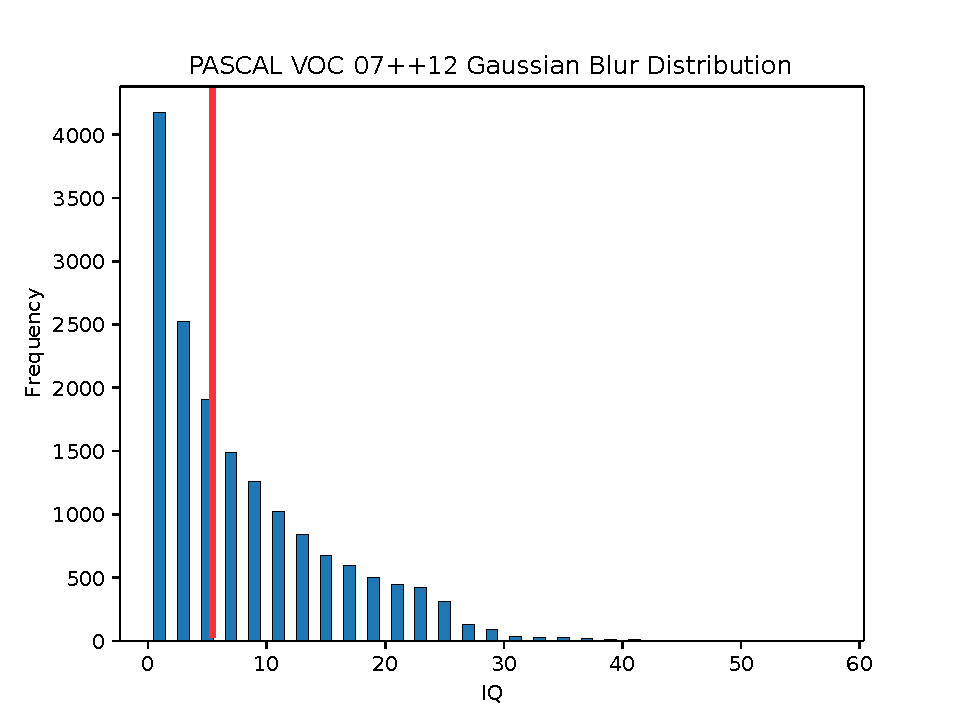
\includegraphics[width=0.5 \textwidth]{figs/GaussianBlurdistred.pdf}
    \end{figure}
    \vspace{-0.5cm}
    \begin{figure}
        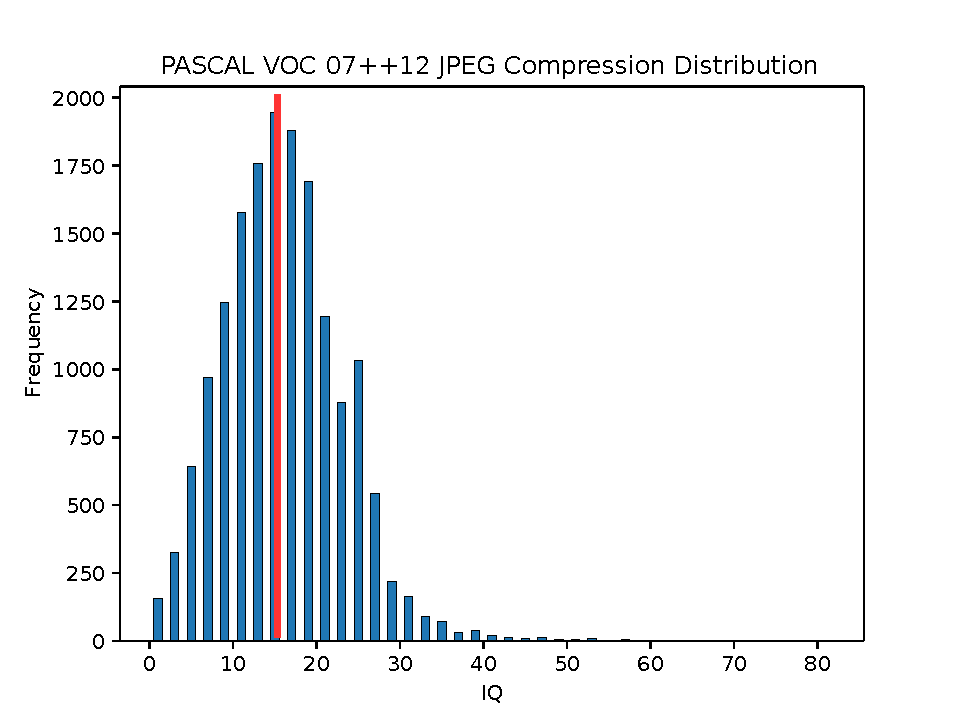
\includegraphics[width=0.5 \textwidth]{figs/JPEGCompressiondistred.pdf}
    \end{figure}

    \column{0.5\textwidth}
    \vspace{-0.5cm}
      \begin{figure}
        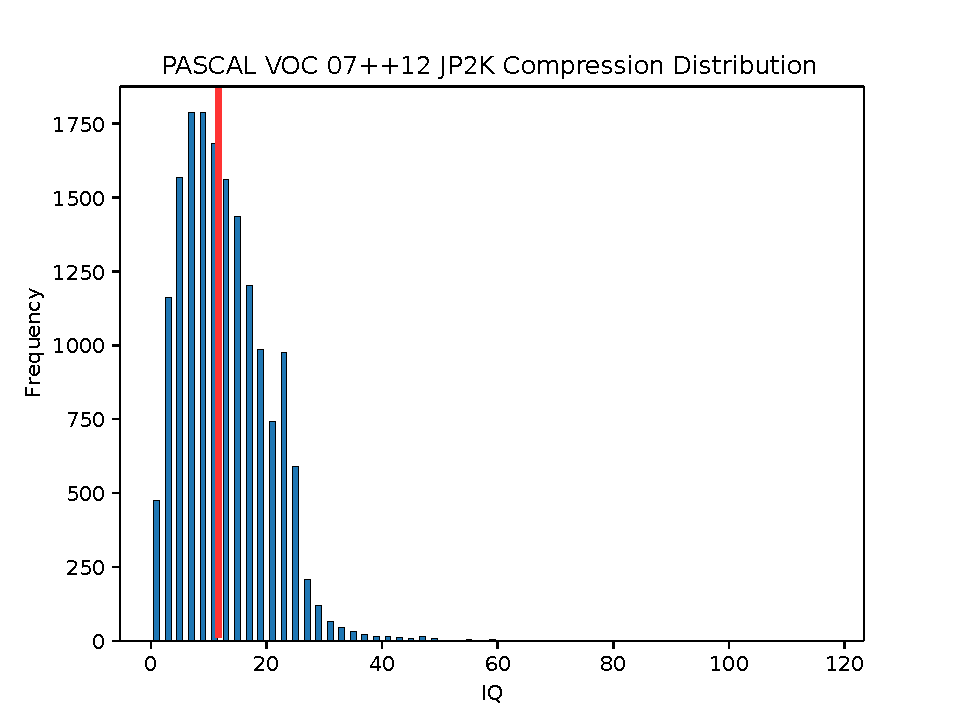
\includegraphics[width=0.5 \textwidth]{figs/JP2KCompressiondistred.pdf}
    \end{figure}
    \vspace{-0.5cm}
    \begin{figure}
        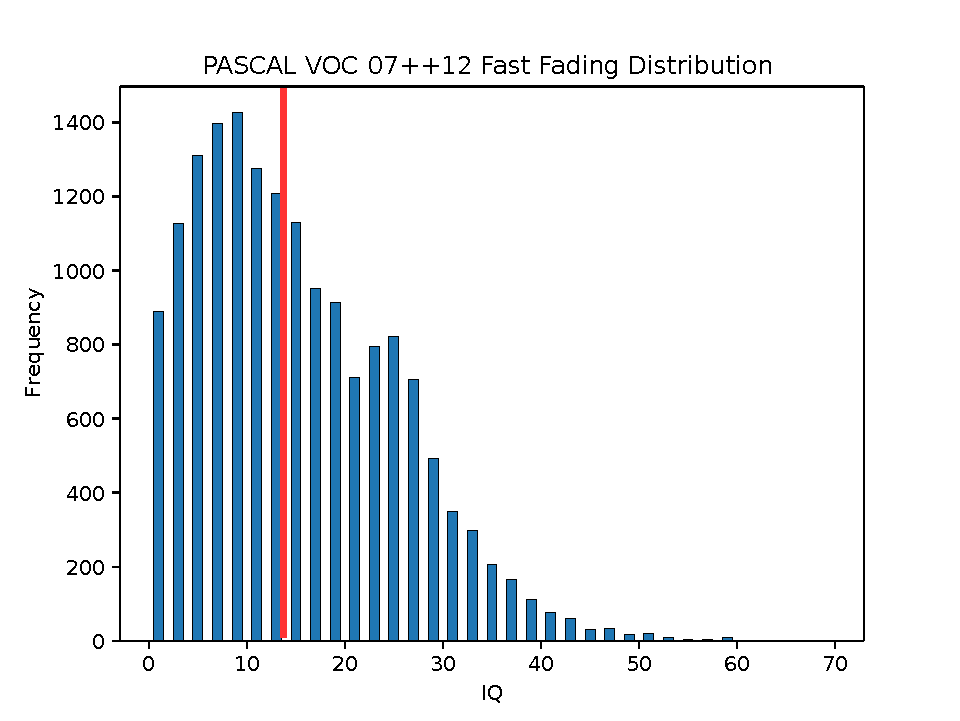
\includegraphics[width=0.5 \textwidth]{figs/FastFadingdistred.pdf}
    \end{figure}
    \end{columns}
\end{frame}

\begin{frame}{Ensemble Combination}{General Overview}
\begin{columns}
    \column{0.5\textwidth}
        \begin{block}{Combining detections}
        \begin{itemize}
            \item 5 ensemble factors, 10 ensemble members
            \item Each factor weighted equally
            \item Combine bounding box and confidence
        \end{itemize}
    \end{block}
    \column{0.5\textwidth}
        \begin{figure}
            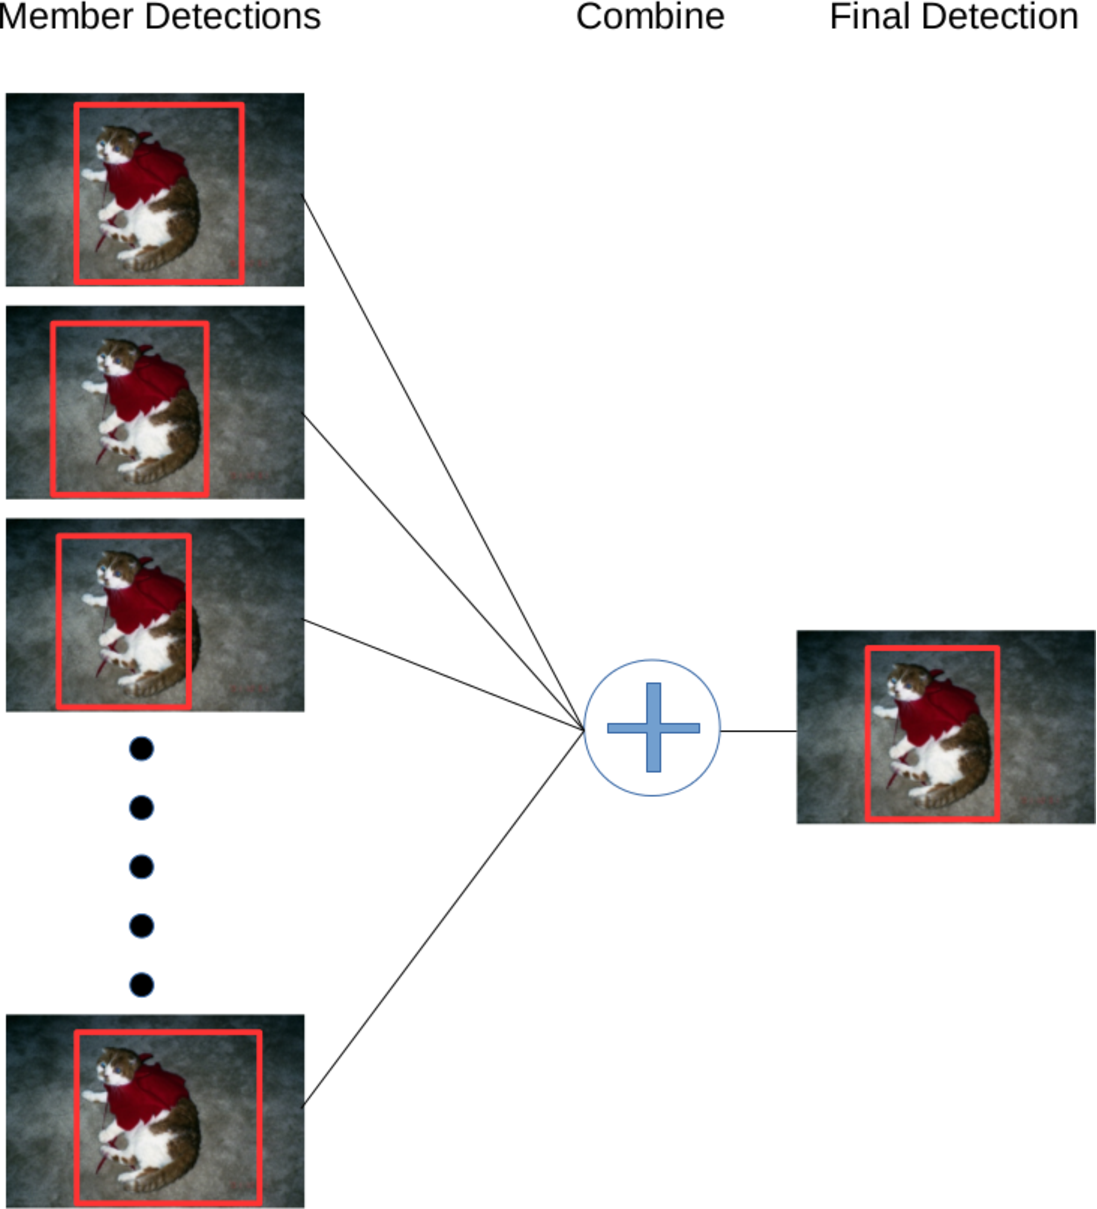
\includegraphics[width=1.0 \textwidth]{figs/ensemble.pdf}
        \end{figure}
    \end{columns}
\end{frame}



\begin{frame}{Ensemble Combination}{Average Ensemble}
\begin{columns}
    \column{0.5\textwidth}
        \begin{block}{Averaging detections}
        \begin{itemize}
            \item For each factor measure in relation to training data
            \item Pick appropriate model detection
            \item Average 5 detections
        \end{itemize}
    \end{block}
    \column{0.5\textwidth}
        \begin{figure}
            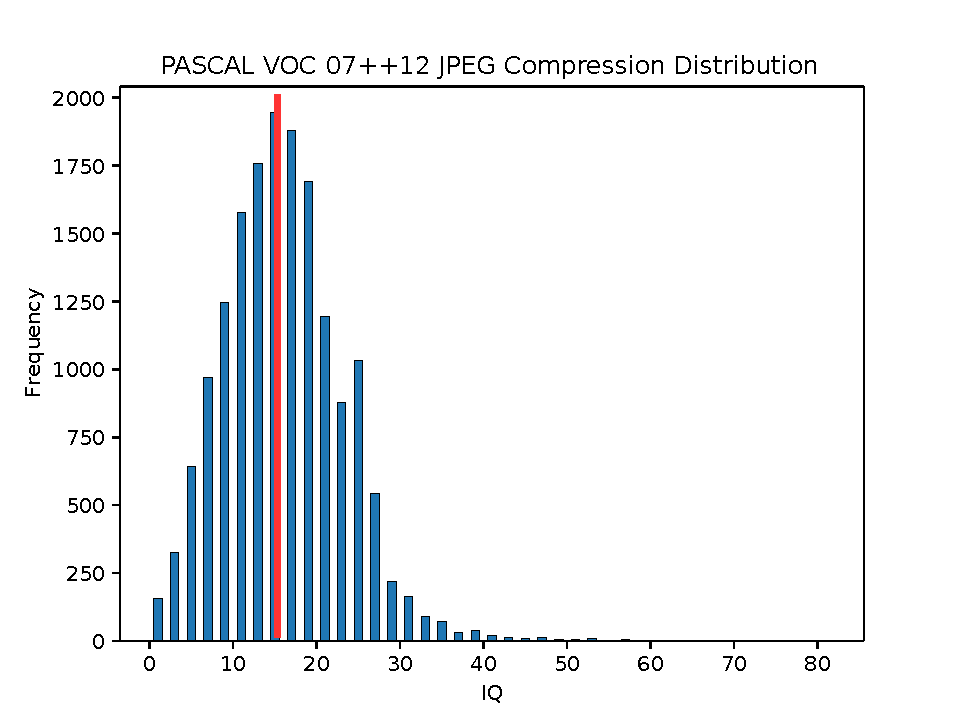
\includegraphics[width=1.0 \textwidth]{figs/JPEGCompressiondistred.pdf}
        \end{figure}
    \end{columns}
\end{frame}

\begin{frame}{Ensemble Combination}{Weighted Average Ensemble}
\begin{columns}
    \column{0.5\textwidth}
        \begin{block}{Weighted averaging detections}
        \begin{itemize}
            \item For each factor and network measure in relation to training data
            \item Weigh detection according to a normalised measurement
            \item Average up to 10 weighted detections
        \end{itemize}
    \end{block}
    \column{0.5\textwidth}
        \begin{figure}
            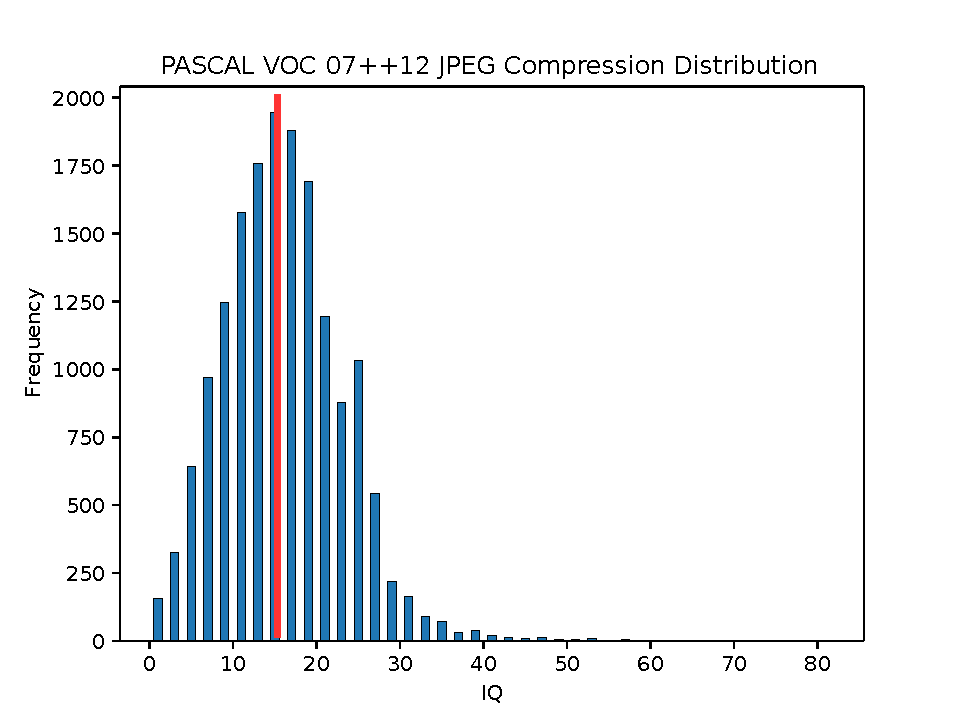
\includegraphics[width=1.0 \textwidth]{figs/JPEGCompressiondistred.pdf}
        \end{figure}
    \end{columns}
\end{frame}
